%PIP-412029OA046
\documentclass[reprint,amsmath,amssymb,aps,prb,footinbib,floatfix]{revtex4-2}
\bibliographystyle{apsrev4-2}
\usepackage{afterpage}
\usepackage{blindtext}
\usepackage[rgb]{xcolor}
%\usepackage[twocolumn=true,includehead=false,left=.75in,right=.75in,top=.75in,bottom=.75in]{geometry}
%\usepackage[letterpaper, portrait, twocolumn, twoside, left=2cm, hmarginratio=2:1, includemp, marginparwidth=43pt, bottom=1cm, foot=.7cm, includefoot, textheight=11cm, heightrounded, columnsep=1cm, dvips, verbose]{geometry}
\definecolor{Cred}{RGB}{208, 32, 46}
\usepackage[firstpage=true]{background}
\usetikzlibrary{calc}
%\usepackage{tikz}
\backgroundsetup{angle = 0, scale = 1, vshift = 0pt, opacity=1,
  contents = {\begin{tikzpicture}[overlay,remember picture]
    \node at (0,0) {\includegraphics[scale=1]{EC_RC.pdf}};
\end{tikzpicture}
}
}
%    \draw (3.4in,3.75in) node[inner sep=0] {\includegraphics[width=1in]{arrow.pdf}};
%    \draw (3.5in,3.85in) node[rotate=-90] {\scshape{Editor's}};
%    \draw (3.5in-\baselineskip,3.85in) node[rotate=-90] {\scshape{Suggestion}};
%\end{tikzpicture}

\usepackage{graphicx} % Required for inserting images
\usepackage{mathtools} % Useful for a bunch of math stuff
\usepackage{cleveref} % Use for better cross-references
\usepackage[caption=false]{subfig} % For sub-figures
\usepackage{booktabs} % For nicer looking tables
\usepackage[twoside]{fancyhdr}
\usepackage{appendix}

\usepackage{placeins}




\fancypagestyle{plain}{%
%\setlength{\headheight}{60pt}
\fancyhead[L,C]{}
\fancyhf{}
\fancyhead[R]{\raisebox{.6cm+1pt}{\textbf{Rapid Communication}}}
\fancyhead[L]{ \raisebox{.6cm+1pt}{\scshape{Editor's Suggestion}\vspace{12pt}}}
\fancyhead[C]{\raisebox{.6cm}{\large\scshape{CARTHAGE}}\hspace{0.2cm}\includegraphics[height=1.5cm]{Logo.pdf}\hspace{0.1cm}\raisebox{.6cm}{\large\scshape{COLLEGE 
 }}}
\fancyfoot[C]{\thepage}
\renewcommand{\headrulewidth}{0pt}
\renewcommand{\footrulewidth}{0pt}
}
\usepackage{printlen}


\pagestyle{fancy}
\fancyhf{}
\fancyheadinit{\setlength{\headheight}{20pt}}
\fancyhead[RO,LE]{\textbf{Rapid Communication}}
\fancyhead[LO,RE]{\textit{Phys. in Prog.} \textbf{2} (Feb. 2026)}
\fancyhead[C]{ \large \scshape{PHYSICS IN PROGRESS}}
\fancyfoot[C]{\thepage}
\renewcommand{\headrulewidth}{0.4pt}
\renewcommand{\footrulewidth}{0pt}

% These are packages I am using in this document
\usepackage{siunitx}

% Everything up to here is the 'document preamble'

\begin{document} 

\vspace*{25pt}


\title{Dispersing Doubt: how wavelength affects refraction.}

\author{Skylar Farr}
\affiliation{%
Department of Physics and Astronomy,  Carthage College, 2001 Alford Park Drive, Kenosha, WI 53140, USA
}%
\collaboration{Received January 29, 2026, Published online February 5, 2026}
\begin{abstract}
    A comparison of the index of refraction of two lasers as refracted through the same media will result in the dispersion. By using the Michelson Interferometer experiment to find the wavelengths of various lasers and a semi-cylindrical prism to calculate the indices, the different of the two indices can be taken to get the dispersion of the two different wavelengths from the lasers. The calculated dispersion was $0.014\pm0.13$. This dispersion is consistent with what would be expected from only two separate lasers that were not many wavelengths apart. Given more options for laser colors to analyze, the data would be a lot more accurate.
\end{abstract}


\maketitle
\section{Introduction}
    Indices of refraction, interferometry, wavelength, dispersion. All terms that are encompassed by the field of optics. Each has a rich history and background rooted in curiosity to understand the world around us. Starting with interferometry which was used to find the wavelengths of light and other forms of waves \cite{hariharan2010basics}. Albert A. Michelson, an American physicist, invented the Michelson Interferometer in order to prove the existence of the aether. He ended up with null results, but post this invention, it has been used consistently to measure wavelengths of light and, in the case of this experiment, lasers. Different types of lasers have different wavelengths, this fact does not affect the interferometry process but it does affect indices of refraction. An index of refraction is the ratio of the speed of light in two different media and it determines how much that light is bent or refracted when entering a material \cite{stachura2024fermat}. For differences in wavelength, despite having consistent media when measuring the values, the indices will vary. This variation is called dispersion. Dispersion is the scattering of light away from its central point or into multiple different components. Dispersion is relatively simple to understand but it can be used in many complicated systems and it is important for understanding the behavior of different waves. It is very important for types of imaging to ensure that light does not bleed and that the image being displayed is sharp and clear. Additionally, it can be used in fiber-optic communication systems.


\section{Red vs. Green}
    Observing dispersion through a medium depends on two things, the wavelength of the light or laser being used, and the index of refraction of the medium. Both of these variables can be measured experimentally. To determine the wavelength, an experiment can be performed using a Michelson Interferometer as seen in Fig. \ref{wavelength schematic}.  The equipment used for this experiment was the PASCO Model OS-8501 Interferometer and it works by splitting a laser beam and reflecting it off of a stationary and movable mirror onto a viewing screen where the fringes of the wave are visible, as seen in Fig. \ref{double}. From here, the movable mirror can be adjusted in micron graduations which causes the fringes on the viewing screen to change. By measuring the distance the mirror is moved, and comparing it to the number of fringes that pass on the viewing screen, the wave length can be calculated using this equation,
    \begin{equation}
        \lambda=\frac{2d}{m},
    \end{equation}
    where $\lambda$ is the wavelength, $d$ is the distance M2 is moved, and $m$ is the number of fringes counted.

    \begin{figure}
        \centering
        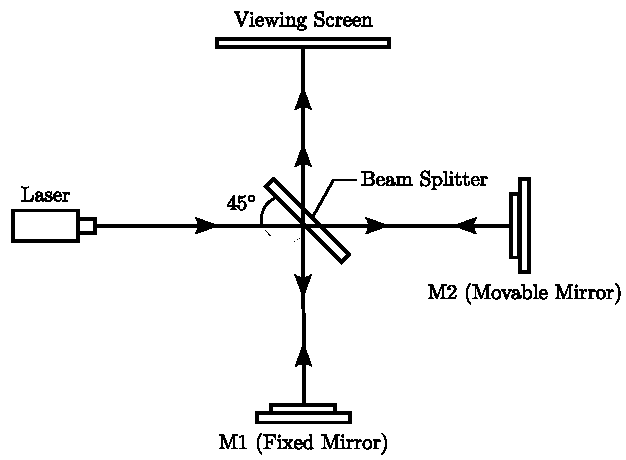
\includegraphics[width=0.9\linewidth]{Wavelength Schematic.pdf}
        \caption{Schematic of a Michelson Interferometer. A laser is shone into a beam splitter angled at $45^\circ$ where it is reflected off of a fixed mirror $M1$ and a movable mirror $M2$, onto a viewing screen where the fringes of the wave are visible.}
        \label{wavelength schematic}
    \end{figure}

    \begin{figure*}[t]
    \centering
    \subfloat[Fringes of red laser.]{%
        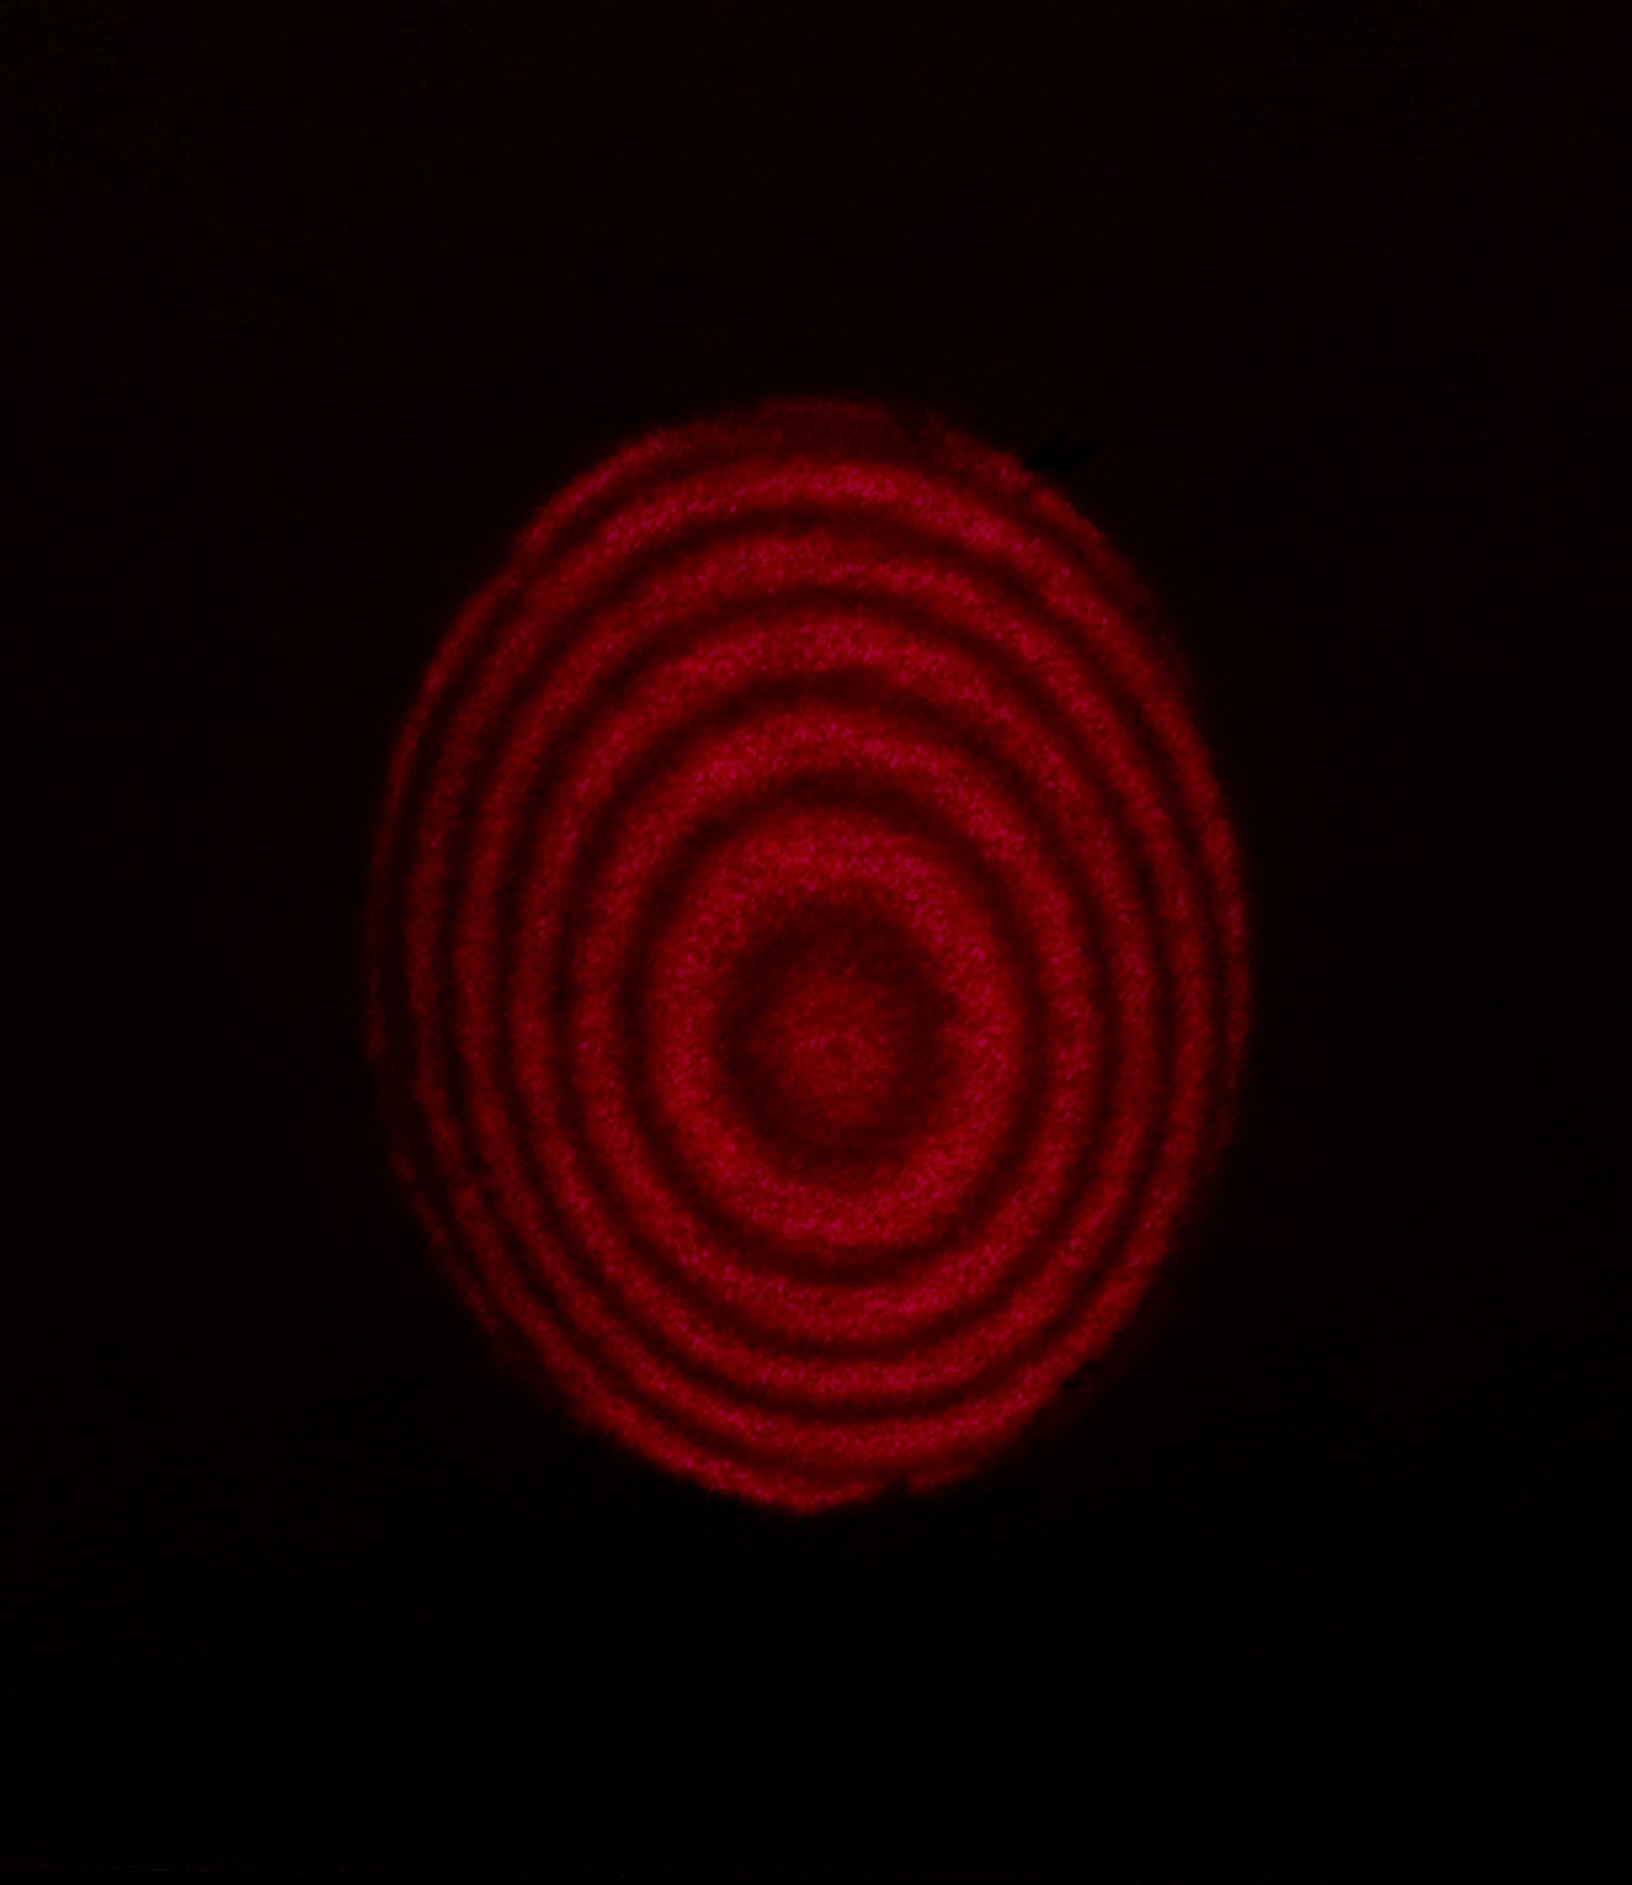
\includegraphics[width=0.5\columnwidth]{Red Laser_Interferometer.jpg}%
    }\hskip 0.05\textwidth
    \subfloat[Fringes for green laser.]{%
        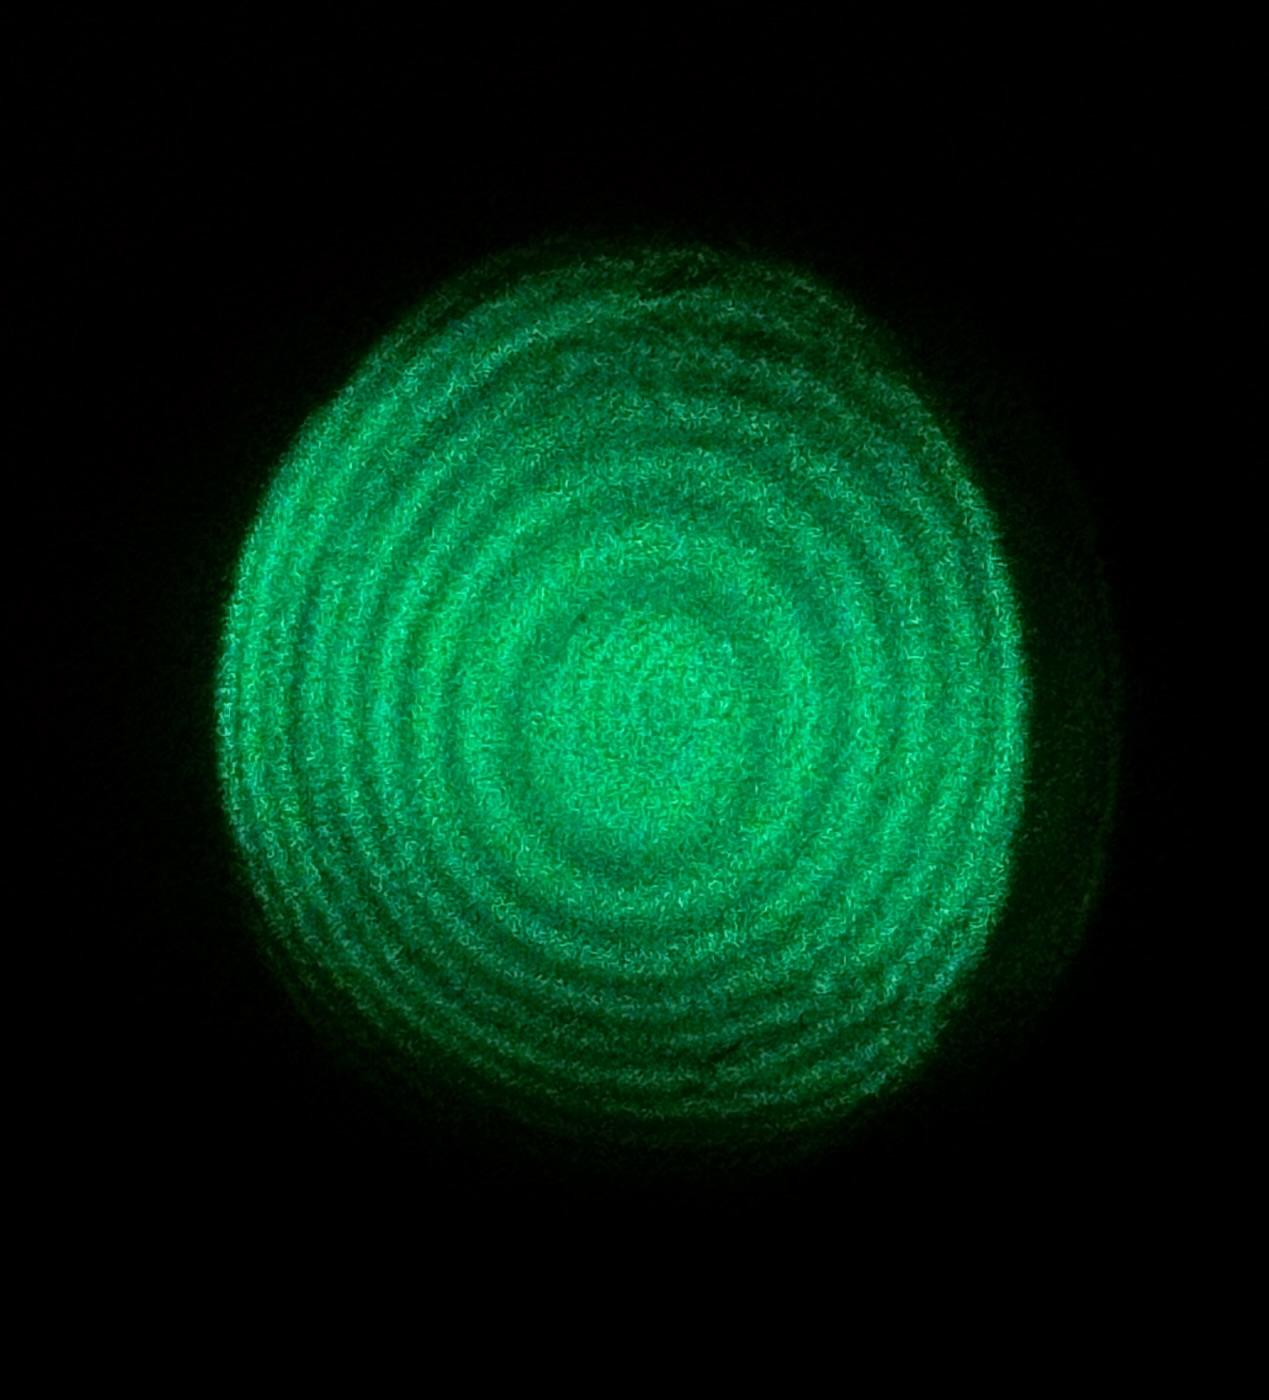
\includegraphics[width=0.524\columnwidth]{Green Laser_Interferometer.jpg}%
    }
    \caption{{The resulting projection of the laser after it has gone through the Michelson Interferometer.}}
    \label{double}
    \end{figure*}

    Once the wavelengths are calculated the indices of refraction can be calculated. This is done by using Snell's Law to find the index of refraction of the medium the lasers are passing through. Snell's Law is
    \begin{equation}
        n_1\sin(\theta_1)=n_2\sin(\theta_2),
    \end{equation}
    where $n_1$ is the index of refraction of the first medium the laser passes through, which in this case is air at a value of $n_1\approx1$, $\theta_1$ is the angle of incidence, or the angle that the laser enters the second medium at, $\theta_2$ is the outgoing angle, and $n_2$ is the index of refraction of the second medium which is the value that is in the process of being calculated. This experimental set up contains a graduated ray table, and a semi-cylindrical acrylic or PMMA plastic prism as seen in Fig. \ref{index schematic}.

    \begin{figure}
        \centering
        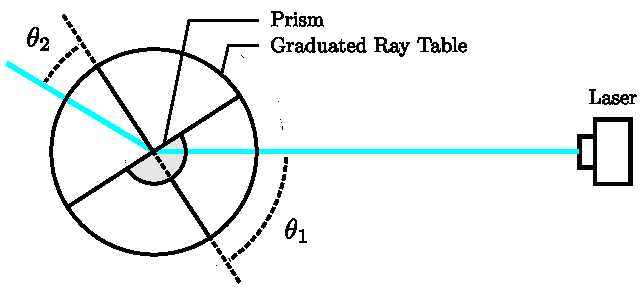
\includegraphics[width=0.8\linewidth]{Index Schematic.pdf}
        \caption{Schematic of the index of refraction experiment. The laser is directed into the semi-cylindrical prism placed on top of the graduated ray table. The ray table is rotated to the angle of incidence $\theta_1$ which produces the outgoing angle $\theta_2$.}
        \label{index schematic}
    \end{figure}

    For both of the separate experiments, two sets of data were taken; once for a red laser and once for a green laser. The red laser is a PASCO OS-8525A Basic Optics Red Diode Laser with a wavelength $\lambda_r=650$ nm, and the green laser is a PASCO OS-8458B Basic Optics Green Diode Laser with a wavelength of $\lambda_g=515$ nm. After both sets of data were taken, each experiment went through specified linear regressions and error analysis. The estimated uncertainty for the wavelength of both lasers was $\delta=\pm$ \SI{1}{\micro\metre}. The estimated uncertainty for the index of the red laser was $\delta_r=\pm3^\circ$ and the green laser was $\delta_g=\pm2^\circ$. These uncertainties were used in the error propagation of the data sets.

    Starting with wavelength. The calculated wavelength based on the slope of the plotted data in Fig. \ref{graph wavelengths}, is $\lambda_r=697\pm14$ nm for the red laser, while green is $\lambda_g=546\pm14$ nm. These values for wave length are consistent in showing the behavior of a wave when it is measured by a Michelson Interferometer, but the data is not accurate when compared to the measured wavelengths of both lasers. This is a little bit surprising but not completely unexpected. When the knob that controlled the movement of M2 was rotated it would often continue to move slightly in the opposite direction that it had been spun once it was let go since it was spring loaded. This cause a few instances of having to completely restart during the counting of the number of fringes or it moved with out being noticed and the fringes were miscounted.

    \begin{figure}
        \centering
        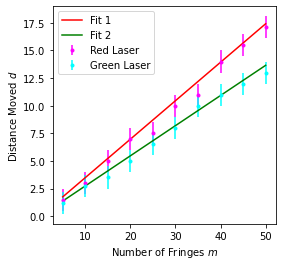
\includegraphics[width=0.8\linewidth]{Graph of Wavelengths.png}
        \caption{Number of fringes vs. distance moved. Graph of the slope of each laser after a linear regression to determine the wavelength. Error bars are based off of the estimated uncertainty.}
        \label{graph wavelengths}
    \end{figure}

    Now that the wavelength data has been analyzed and the wavelengths have been found, the index of refraction can be found. The purpose of finding the wavelength before the index of refraction was to understand the difference in properties of the two lasers, under the assumption the recorded values were not available. The calculated indices based on the slop of the data plotted in Fig. \ref{graph indicies}, is $n_r=1.52\pm0.08$ for the red laser, and $n_g=1.51\pm0.05$ for the green laser. These values are relatively close to the recorded values of the index of refraction for the respective lasers \cite{sultanova2009dispersion}. Despite any errors, these data sets successfully show the expected behavior of the index of refraction through acrylic.

    \begin{figure}
        \centering
        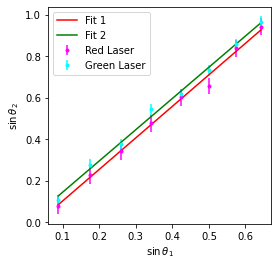
\includegraphics[width=0.8\linewidth]{Graph of Indicies.png}
        \caption{Graph of $\sin(\theta_1)$ vs $\sin(\theta_2)$, where the slope of each laser is plotted with a best fit after linear regression to determine the index of refraction. The error bars are based off of the estimated uncertainty.}
        \label{graph indicies}
    \end{figure}

     The last, but most important step, is calculating the dispersion. This is done by taking the difference of two indices, and calculating the uncertainty from the uncertainties of the two indices as seen below
     \begin{align}
         \Delta n &= n_r-n_g, & \delta_n &= \delta_r+\delta_g,
     \end{align}
     which for this data gives, $\Delta n=0.014\pm0.13$. While this may look like an extremely bad number due to the uncertainty being larger than the calculated value, its actually pretty normal. Since the dispersion is being found with only two wavelengths that are already close in number, it is not surprising that the dispersion is so small. Since you can only add uncertainties not subtract despite the original equation needing subtraction, it just grows.

\section{Conclusion}
    As it has been found, dispersion can often be an incredibly small number with a high uncertainty which makes precision important whenever it comes to using dispersion in any application. It is very simple to find, as long as you have all the right components, but taking a measurement that is truly accurate and precise takes a lot of time and patience. Within both experiments, there were a lot of opportunities for error and as much of that error was taken into account as possible. Comparatively, the data here is not very accurate because of the difference between the recorded and measured values, but the behaviors of the data aligned with what was expected. This kind of error can be systemic, there could be something wrong with the equipment being used. The age of the equipment could have caused it do degrade over time. Another systemic error could be a problem with the person taking the data. It is possible that the data was consistently misread the same way every time data was recorded.

    Again, regardless of any inaccuracy, this experiment was still able to take somewhat reasonable numbers and calculate a dispersion between a red and green laser as it is seen through an acrylic prism. The experiment has really reflected how much every part of optics feeds into each other and any doubts that previously plagued the minds of readers is, ideally, dispersed.


\section*{Acknowledgments}
This research would not have been made possible without funding from the Carthage College Physics and Astronomy Department along with assistance from Dr. Joseph Anderson.

\section*{Data Availability Statement}
A Jupyter notebook containing all the experimental data, data analysis, figure generation, and additional information on uncertainty analysis can be found in the supplemental materials. \footnote{See online article posting for access to supplemental material.}


\bibliography{bib}

\end{document}